\documentclass[12pt,a4paper]{report}
\usepackage{amssymb,amsthm,amsmath,amscd}
\usepackage{latexsym}
\usepackage{enumerate}
\usepackage[german]{babel}
\usepackage{verbatim}
\usepackage[utf8]{inputenc}
\usepackage{hyperref}
\usepackage{graphicx}



\begin{document}
% ---------------

\begin{titlepage}
	\begin{center}
		
		\vspace*{1.0cm}
		\huge
		\textsc{\bf{PS Netze und Verteilte Systeme}}
		
		\vspace*{4.0cm}
		\textsc{
			\normalsize{eingereicht von} \\[0.5\baselineskip]
			{\large Baumgartner Dominik}
		}
		
		\vspace*{3.0cm}
		\textsc{
			\normalsize{Gruppe 1(13:00)}
		}
		
	\end{center}
	
\end{titlepage}

\ \\
\textbf{Aufgabe 25:}
\\
\\
Wie funktioniert die Konfiguration von Ipv6-Geräten und welche Rolle spielen ICMPv6 und das
Neighbor Discovery Protocol dabei?
\\
Ein IPv6-Host kann mehrere IPv6-Adressen haben. Wenn IPv6 im Host aktiviert ist, dann hat er zumindest eine link-lokale bzw. verbindungslokale Adresse. Wenn zusätzlich der Netzzugang und der Netzzugangsrouter IPv6-fähig sind, dann hat ein Host noch eine zweite IPv6-Adresse. Das ist die globale Adresse. Wenn Privacy Extensions im Host aktiviert ist, dann hat er noch zusätzlich eine temporäre globale Adresse, die für externe Verbindungen genutzt wird. Da temporäre Adressen irgendwann ihre Gültigkeit verlieren, kann ein Host auch mehrere temporäre Adressen haben. Zu einer vollständigen IPv6-Konfiguration gehören aber nicht nur die IPv6-Adressen des Hosts, sondern mindestens noch die IPv6-Adressen des Standard-Gateways und eines DNS-Servers.
\\
\\
Link-Lokale Adresse:\\
Standardmäßig ist es so, dass wenn ein IPv6-Client gestartet wird, dann weist er sich selber eine link-lokale IPv6-Adresse zu. Verbindungen in andere Netze, zum Beispiel ins Internet, sind mit einer link-lokalen IPv6-Adresse nicht möglich. Sie ist nur im lokalen Netz gültig.
\\
Die ersten 64 Bit einer link-lokalen IPv6-Adresse sind fest vorgegeben. Davon sind die ersten 16 Bit "fe80". Weitere 48 Bit werden mit Nullen aufgefüllt. Die restlichen 64 Bit der IPv6-Adresse entsprechen dem Interface Identifier für den die MAC-Adresse des Netzwerkadapters herangezogen wird. Dabei wird die 48-Bit-MAC-Adresse in der Mitte mit einem "ff:fe" aufgefüllt, damit eine Länge von 64 Bit entsteht. Zusätzlich wird das zweite Bit im ersten Byte invertiert.
Dieses Verfahren gehört zur Stateless Address Autoconfiguration (SLAAC).
\\
\\
Temporären globalen IPv6-Adressen:\\
Die temporären globalen IPv6-Adressen basieren auf den Privacy Extensions. Hierbei wird der globale Präfix verwendet und der ursprüngliche Interface Identifier, der aus der MAC-Adresse gebildet wird, wird durch einen pseudozufälligen Interface Identifier ersetzt. Der wird regelmäßig geändert, um den Datenschutz zu gewährleisten.
\\
\\
Standard Gateway:\\
Im Rahmen der Router Advertisements wird nicht nur der globale Präfix, sondern auch die IPv6-Adresse des Standard-Gateways kommuniziert. Das ist ein Bestandteil von SLAAC.
\\
\\
DNS:
IPv6-Protokoll konfiguriert sich automatisch, ohne dass dabei ein Protokoll wie DHCP (Dynamic Host Configuration Protocol) zum Einsatz kommen muss (SLAAC). 
Alternativ kann die Bekanntgabe der Nameserver-Adresse über DHCPv6 erfolgen.
\\
\\
\textbf{ICMPv6:}
\\
Internet Control Message Protocol for the Internet Protocol Version 6 (ICMPv6). Es dient, wie schon bei IPv4, in Netzwerken zum Austausch von Fehler- und Informationsmeldungen. Zusätzlich findet es aber noch im Neighbor Discovery Protocol, dem Ersatz des Address Resolution Protocol, Verwendung.\\
Im Gegensatz zum ICMP bei IPv4 ist ICMPv6 zwingend für den Betrieb von IPv6 nötig. Ein generelles Blockieren von ICMPv6 auf der Firewall führt dazu, dass IPv6 nicht funktioniert.\\
Auch wenn ICMPv6 auf derselben Netzwerkschicht ist wie IPv6, werden die ICMPv6-Nachrichten vor dem Versenden in IPv6-Pakete eingepackt und so verschickt. Als Protokoll-Nummer wird 58 ins Next-Header-Feld des IPv6-Headers eingefügt.\\
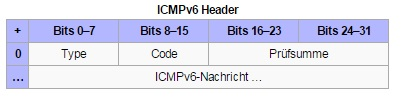
\includegraphics[width=10cm]{icmpv6.jpg}
\\
Das Feld Type gibt die Klasse der ICMP-Nachricht an, welche mit dem Feld Code genauer spezifiziert werden kann. Die Prüfsumme wird zum Prüfen der Gültigkeit des ICMPv6-Pakets benutzt. Der restliche Inhalt der ICMP-Nachricht wird durch den jeweiligen Typ bestimmt. Bei Fehlernachrichten wird nach den möglichen zusätzlichen Feldern immer noch so viel wie möglich vom fehlerverursachenden Paket angehängt.
\\
\\
\textbf{Neighbor Discovery Protocol:}
\\
Neighbor Discovery Protocol (NDP) ist der Ersatz des Address Resolution Protocol (ARP) von IPv4 für IPv6. Es wird unter anderem dazu benutzt, IPv6-Adressen in Link-Layer-Adressen aufzulösen. NDP wird von den am IPv6-Netzwerk beteiligten Knoten benutzt, um die Link-Layer-Adresse von anderen am selben Netzwerk hängenden Knoten ausfindig zu machen und zum Aktualisieren der gecachten Adressen. Für alle nicht am selben Netzwerk hängenden Knoten wird NDP benutzt, um einen/den Router zu finden, der die Pakete weiterleiten kann.\\
\textbf{Funktionsweise:}
\\
Für NDP muss der Knoten für jedes Interface folgende Informationen verwalten:\\
Im Neighbor Cache werden Adressen verwaltet, an die etwas gesendet wurde und die sich im selben Netzwerk befinden. Zu jedem Eintrag einer IPv6-Adresse steht ihre Link-Layer-Adresse. Auch weitere Informationen werden hier verwaltet, wie zum Beispiel Pointer auf Pakete, die auf die Adressauflösung warten, Informationen für die Erreichbarkeitsprüfung oder ob es ein Router ist.\\
Im Destination Cache werden Adressen verwaltet, an die etwas gesendet wurde. Für jeden Eintrag wird, per Link auf den Neighbor Cache, gespeichert, welches der nächste Hop ist, den ein Paket nehmen soll.\\
In der Prefix List werden die Präfixe verwaltet, die auf demselben Netz gültig sind. Jeder Eintrag, außer der zur link-lokalen Adresse, hat ein Ablaufdatum. Somit bleiben nur Netze in der Liste, die von einem Router verkündet werden.\\
In der Default Router List werden alle Router verwaltet, die für das Interface bekannt sind. Die Einträge verweisen auf Einträge im Neighbor Cache. Zusätzlich haben sie ein Ablaufdatum, sodass alte Router verschwinden und nur die erhalten bleiben, die ihre Anwesenheit verkünden.\\
Die Informationen zum Erstellen dieser Listen werden per ICMPv6 ausgetauscht. NDP definiert zu diesem Zweck fünf ICMPv6-Typen.
\\
\\
\textbf{Aufgabe 27:}
\\
\\
Um Applikationen die Nutzung der Netzwerk-Funktionalität eines Betriebssystems zu
ermöglichen, muss eine Schnittstelle definiert werden. Skizzieren Sie das Berkeley-Sockets
Interface und seine wesentlichen Operationen.
\\

% -------------
\end{document}
